\documentclass[a4paper, 12pt]{report}
\usepackage[utf8]{inputenc}
\usepackage[boxed,linesnumbered]{algorithm2e}
\usepackage[bookmarks, breaklinks, colorlinks]{hyperref}
\hypersetup{
	citecolor=black,
	linkcolor=black,
	filecolor=black,
	urlcolor=black
}

\usepackage{graphicx}
\usepackage{pdfpages}
\usepackage{tocbibind}

\def\chapterautorefname{Chapter}


\title{
	\begin{figure}[h]
		\centering
		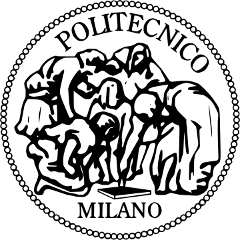
\includegraphics{../common_resources/logo_polimi.png}
	\end{figure}
	\vspace{30px}
	Software Engineering 2 Project: PowerEnJoy \\ \vspace{1em}
	\textbf{D}esign \textbf{D}ocument
}
	

\author{Marco Ieni, Francesco Lamonaca, Marco Miglionico\\Politecnico di Milano, A.A. 2016/2017}
\date{\today\\v1.0}

\begin{document}
\maketitle
\tableofcontents
% \listoffigures
% \listoftables

\chapter{Introduction}
\label{ch:introduction}
\section{Purpose}
This is the Design Document of PowerEnJoy, a digital management system for a car-sharing service that exclusively employs electric cars.
The aim of this document is to show our design choices and the rationale behind them. 

We will analyse the component of the system and how they interact between each other.
Furthermore, we will show the most important algorithms of the project, in order to underline the key aspects of their implementation.
Finally, we will add details to the first description of the user interfaces that was described in the RASD.

\section{Scope}

\section{Definitions, acronyms, abbreviations}
\begin{description}
    \item[JPA:] The Java Persistence API (JPA) is a Java application programming interface specification that describes the management of relational data.
    \item[RASD:] Requirements Analysis and Specification Document.
\end{description}

\section{Reference Documents}
This document refers to the project rules of the Software Engineering 2
project, to the template for the Design Document contained into it and to Requirement Analysis and Specification Document (the previous delivered document)

\section{Document Structure}
This document is divided in five chapters:

\begin{description}

	\item [\autoref{ch:introduction}. Introduction:] It provides a general presentation of the Design document and of the system to be developed.

	\item [\autoref{ch:architectural_design}. Architectural Design:]
	It goes into the detail of the architecture design of the system, describing its basic structure and the interactions of the main subsystems.
	It also contains the architectural style and pattern decisions description.

	\item [\autoref{ch:algorithm_design}. Algorithm Design:] It focuses on the definition of the
most important algorithms of the system, independently from their concrete implementation.

	\item [\autoref{ch:ui_design}. User Interface Design:] It shows how the user interfaces of the system will look like and behave, by means of mock-ups and user experience modelling.
	
	\item [\autoref{ch:requirements_traceability}. Requirements Traceability:] It explains how the requirements we have defined in the RASD map to the design elements that we have defined in this document. 

\end{description}

\chapter{Architectural Design}
\label{ch:architectural_design}
In this chapter we provide a comprehensive view over the system components, both at a physical and logical level.
The system will be firstly described at a very high level, showing the different components and how they interact (section 2.1).
Then the system will be described and detailed in the section 2.2, following a top-down approach.

In section 2.3 we will focus our attention more on the physical level, analysing the deployment of the system on physical tiers, while in section 2.4 we will describe the dynamic behaviour of the system.

Furthermore, section 2.5 will focus on the interface between the different components of the system.
Finally, the design choices and patterns used will be presented and discussed in section 2.6.

\section{Overview}
In this section we will present the high level components of the system and their interaction:

\begin{description}
\item[Mobile application:] This presentation layer consists in the mobile client. It communicates directly with the application server.
\item[Application Server:] This layer contains all the application logic of the system. All the policies, the algorithms and the computation are performed here. This layer offers a service-oriented interface.
\item[Database:] The data layer is responsible for the data storage and retrieval. It does not implement any application logic. This layer must guarantee ACID properties. 
\end{description}

\begin{figure}
	\centering
	\includegraphics[scale=0.6]{architectural_design/Architecture_Diagrams/Layers.png}
	\caption{Layers of the system.}
	\label{fig:layers}
\end{figure}

The system is structured in three layers as we can see in picture \ref{fig:layers}.

This design choice makes it possible to deploy the application server and the database on different tiers. It also improves scalability and fault tolerance.

\begin{figure}
	\centering
	\includegraphics[scale=0.6]{architectural_design/Architecture_Diagrams/Tier.png}
	\caption{Tiers of the system.}
	\label{fig:tiers}
\end{figure}

The figure \ref{fig:tiers}, instead, shows the three tiers from a very high level point of view.

\begin{figure}
	\centering
	\includegraphics[width=\textwidth,height=\dimexpr\textheight-4\baselineskip-\abovecaptionskip-\belowcaptionskip\relax,keepaspectratio]{architectural_design/Architecture_Diagrams/Tier2.png}
	\caption{High level components of the system.}
	\label{fig:high_components}
\end{figure}

The interactions between the main components are shown in the figure \ref{fig:high_components}.

\begin{figure}
    \vspace*{-2cm}
    \makebox[\linewidth]{
        \includegraphics[width=1.3\linewidth]{architectural_design/Architecture_Diagrams/Tier3.png}
    }
    \caption{Description of the tiers, detailed with Java EE components.}
	\label{fig:tiers_description}
\end{figure}

A more detailed description of the three different tiers is shown in picture \ref{fig:tiers_description}.



\section{Component View}
\subsection{Database}
The database tier runs MySQL Community Edition and uses InnoDB as storage engine: the DBMS is fully transactional with rollback and commit, besides it ensure ACID properties and provides automatic recovery from crashes via the replay of logs.

The DBMS will not be internally designed because it is an external component used as a “black box” offering some services: it only needs to be configured and tuned in the implementation phase.
The database can communicate only with the business logic tier using the standard network interface, described in section 2.6. 

Security restrictions will be implemented to protect the data from unauthorized access: the database must be physically protected and the communication has to be encrypted.
Access to the data must be granted only to authorized users possessing the right credentials and system privileges allow only administrators to perform administrative actions in the database, including privileges such as: create database, create procedure, create view, backup database, create table, and execute.

Every software component that needs to access the DBMS must do so with the minimum level of privilege needed to perform the operations. All the persistent application data is stored in the database.
The conceptual design of the database is illustrated by the ER diagram.

Foreign key constraints and triggers are not used: the dynamic behaviour of the data is handled entirely by the Java Persistence API in the Business Application tier.

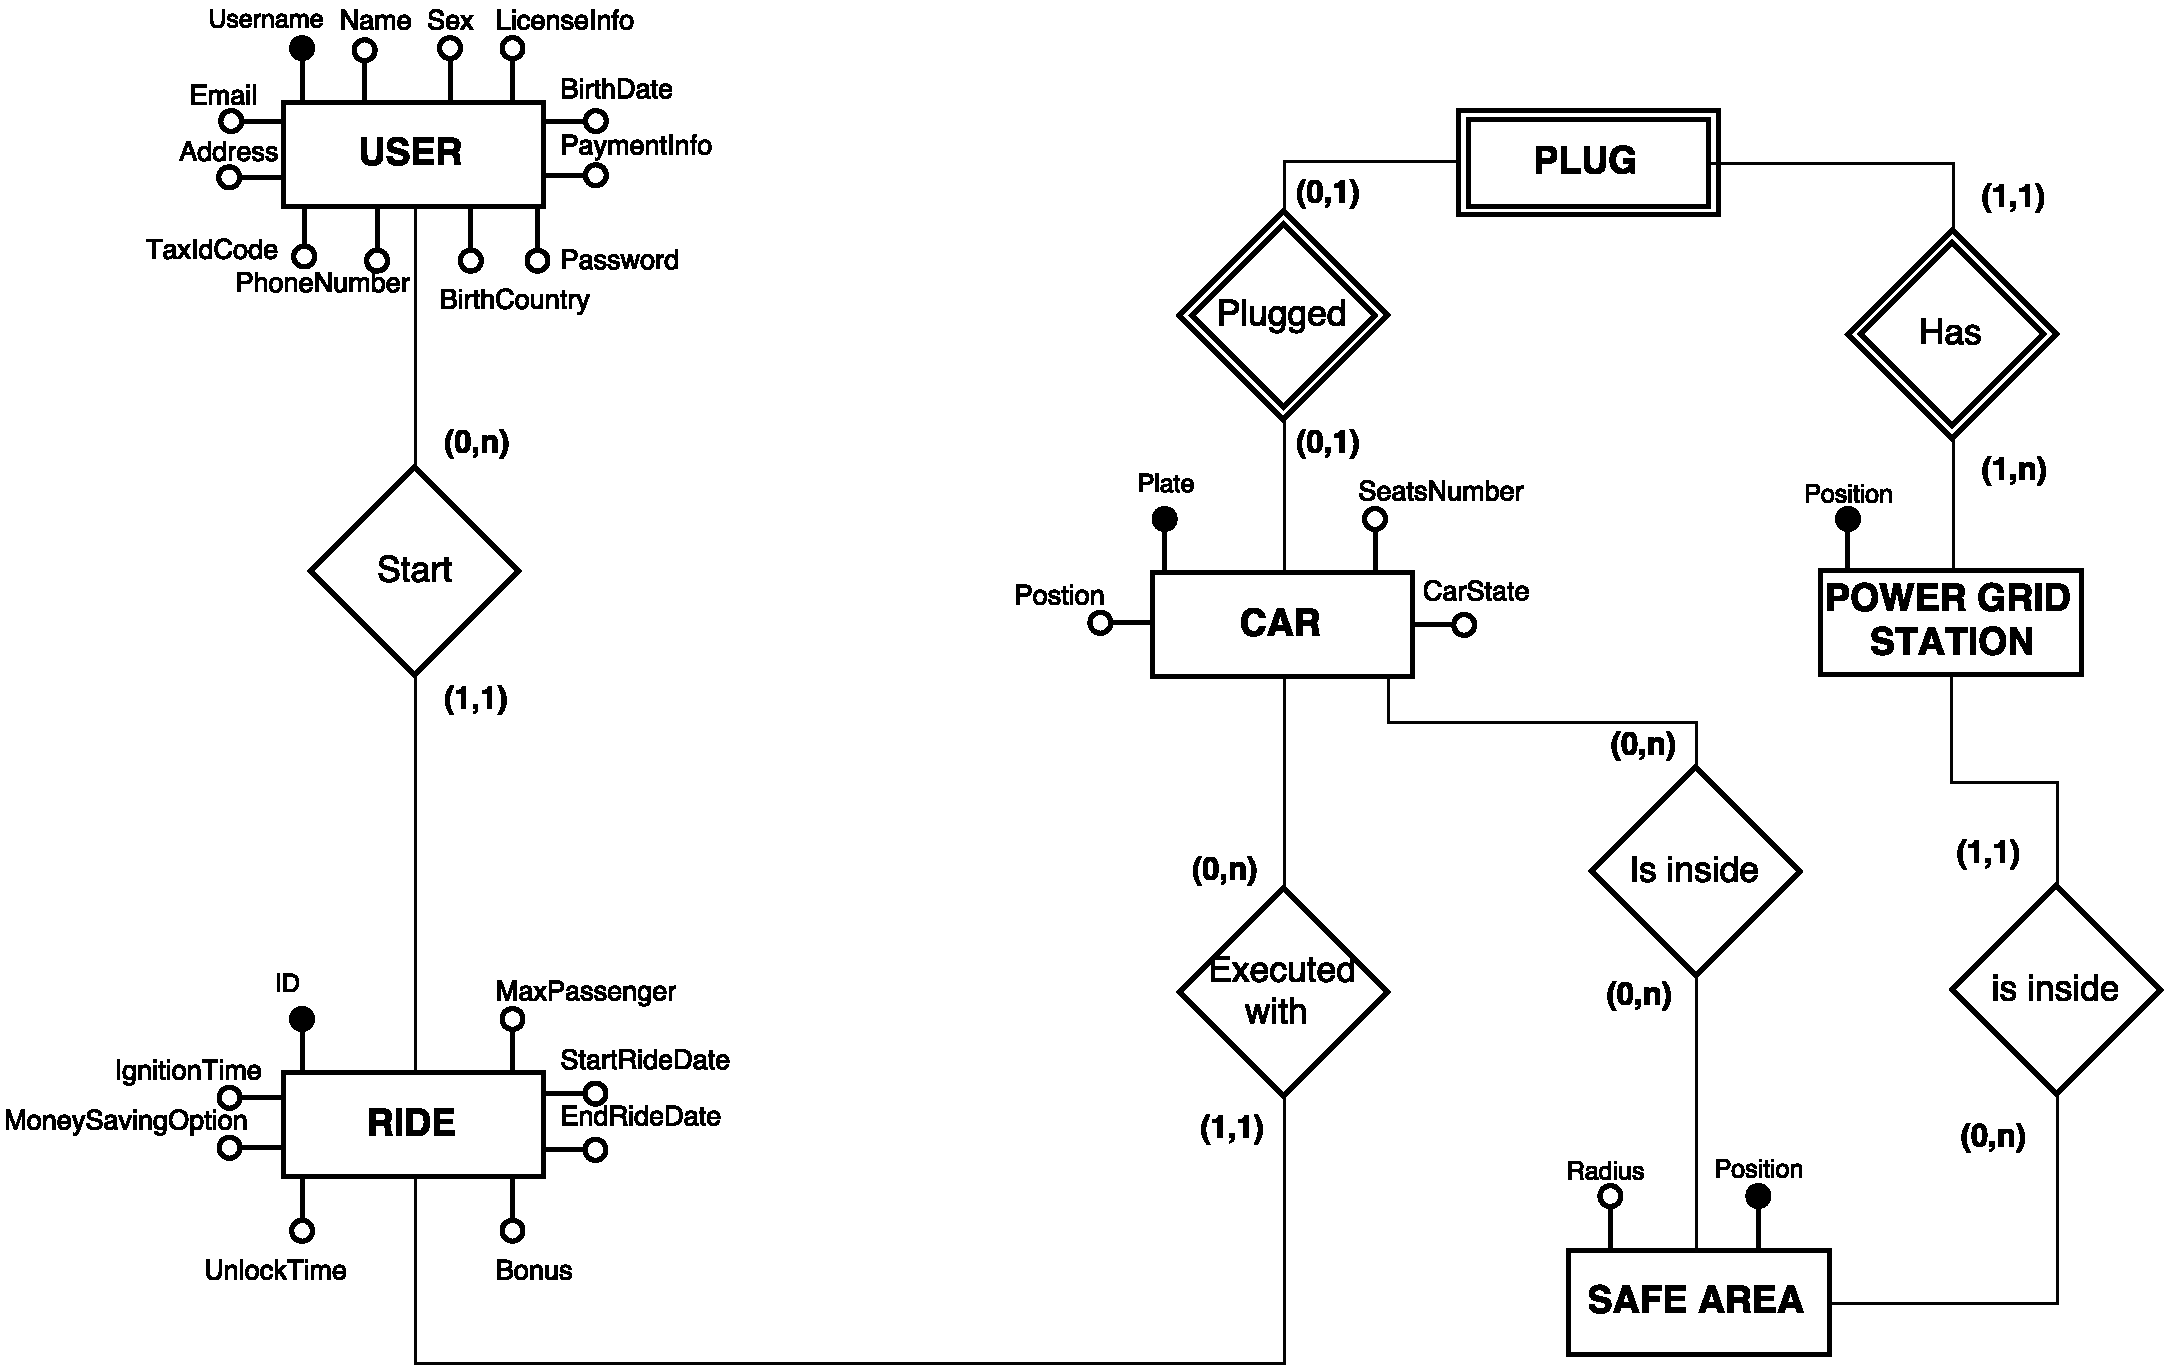
\includepdf{architectural_design/Architecture_Diagrams/ERDiagram.pdf}

\subsection{Application Server}
The application server is implemented in the business logic tier, it runs on an open-source application server, GlassFish, that use Java EE and supports Enterprise JavaBeans.
The access to the DBMS is not implemented with direct SQL queries but using Java Persistence API (JPA), in particular the Java Persistence Query Language (JPQL) makes queries against entities stored in DBMS.
Queries resemble SQL queries in syntax, but operate against entity objects rather than directly with database tables.
The object-relation mapping is done by entity beans.

The Entity Beans representing the database entities are strictly related to the entities of the ER diagram,the data  are stored automatically using container-managed persistence.
They are persistent because their data is stored persistently in the database and they do survive a server failure, failover, or a network failure.
The business logic is implemented by custom-built stateless Enterprise JavaBeans (EJB).

Our application is quite simple, the state of the cars is stored in the DB, so we do not need stateful EJBs which can be more expensive,but just stateless EJBs.
Concurrency management and performance are fundamental, so the reuse of EJBs for many requests is a desirable behaviour.
The application server implements a RESTful API using JAX-RS to allow the clients to use the services offered by the EJBs.
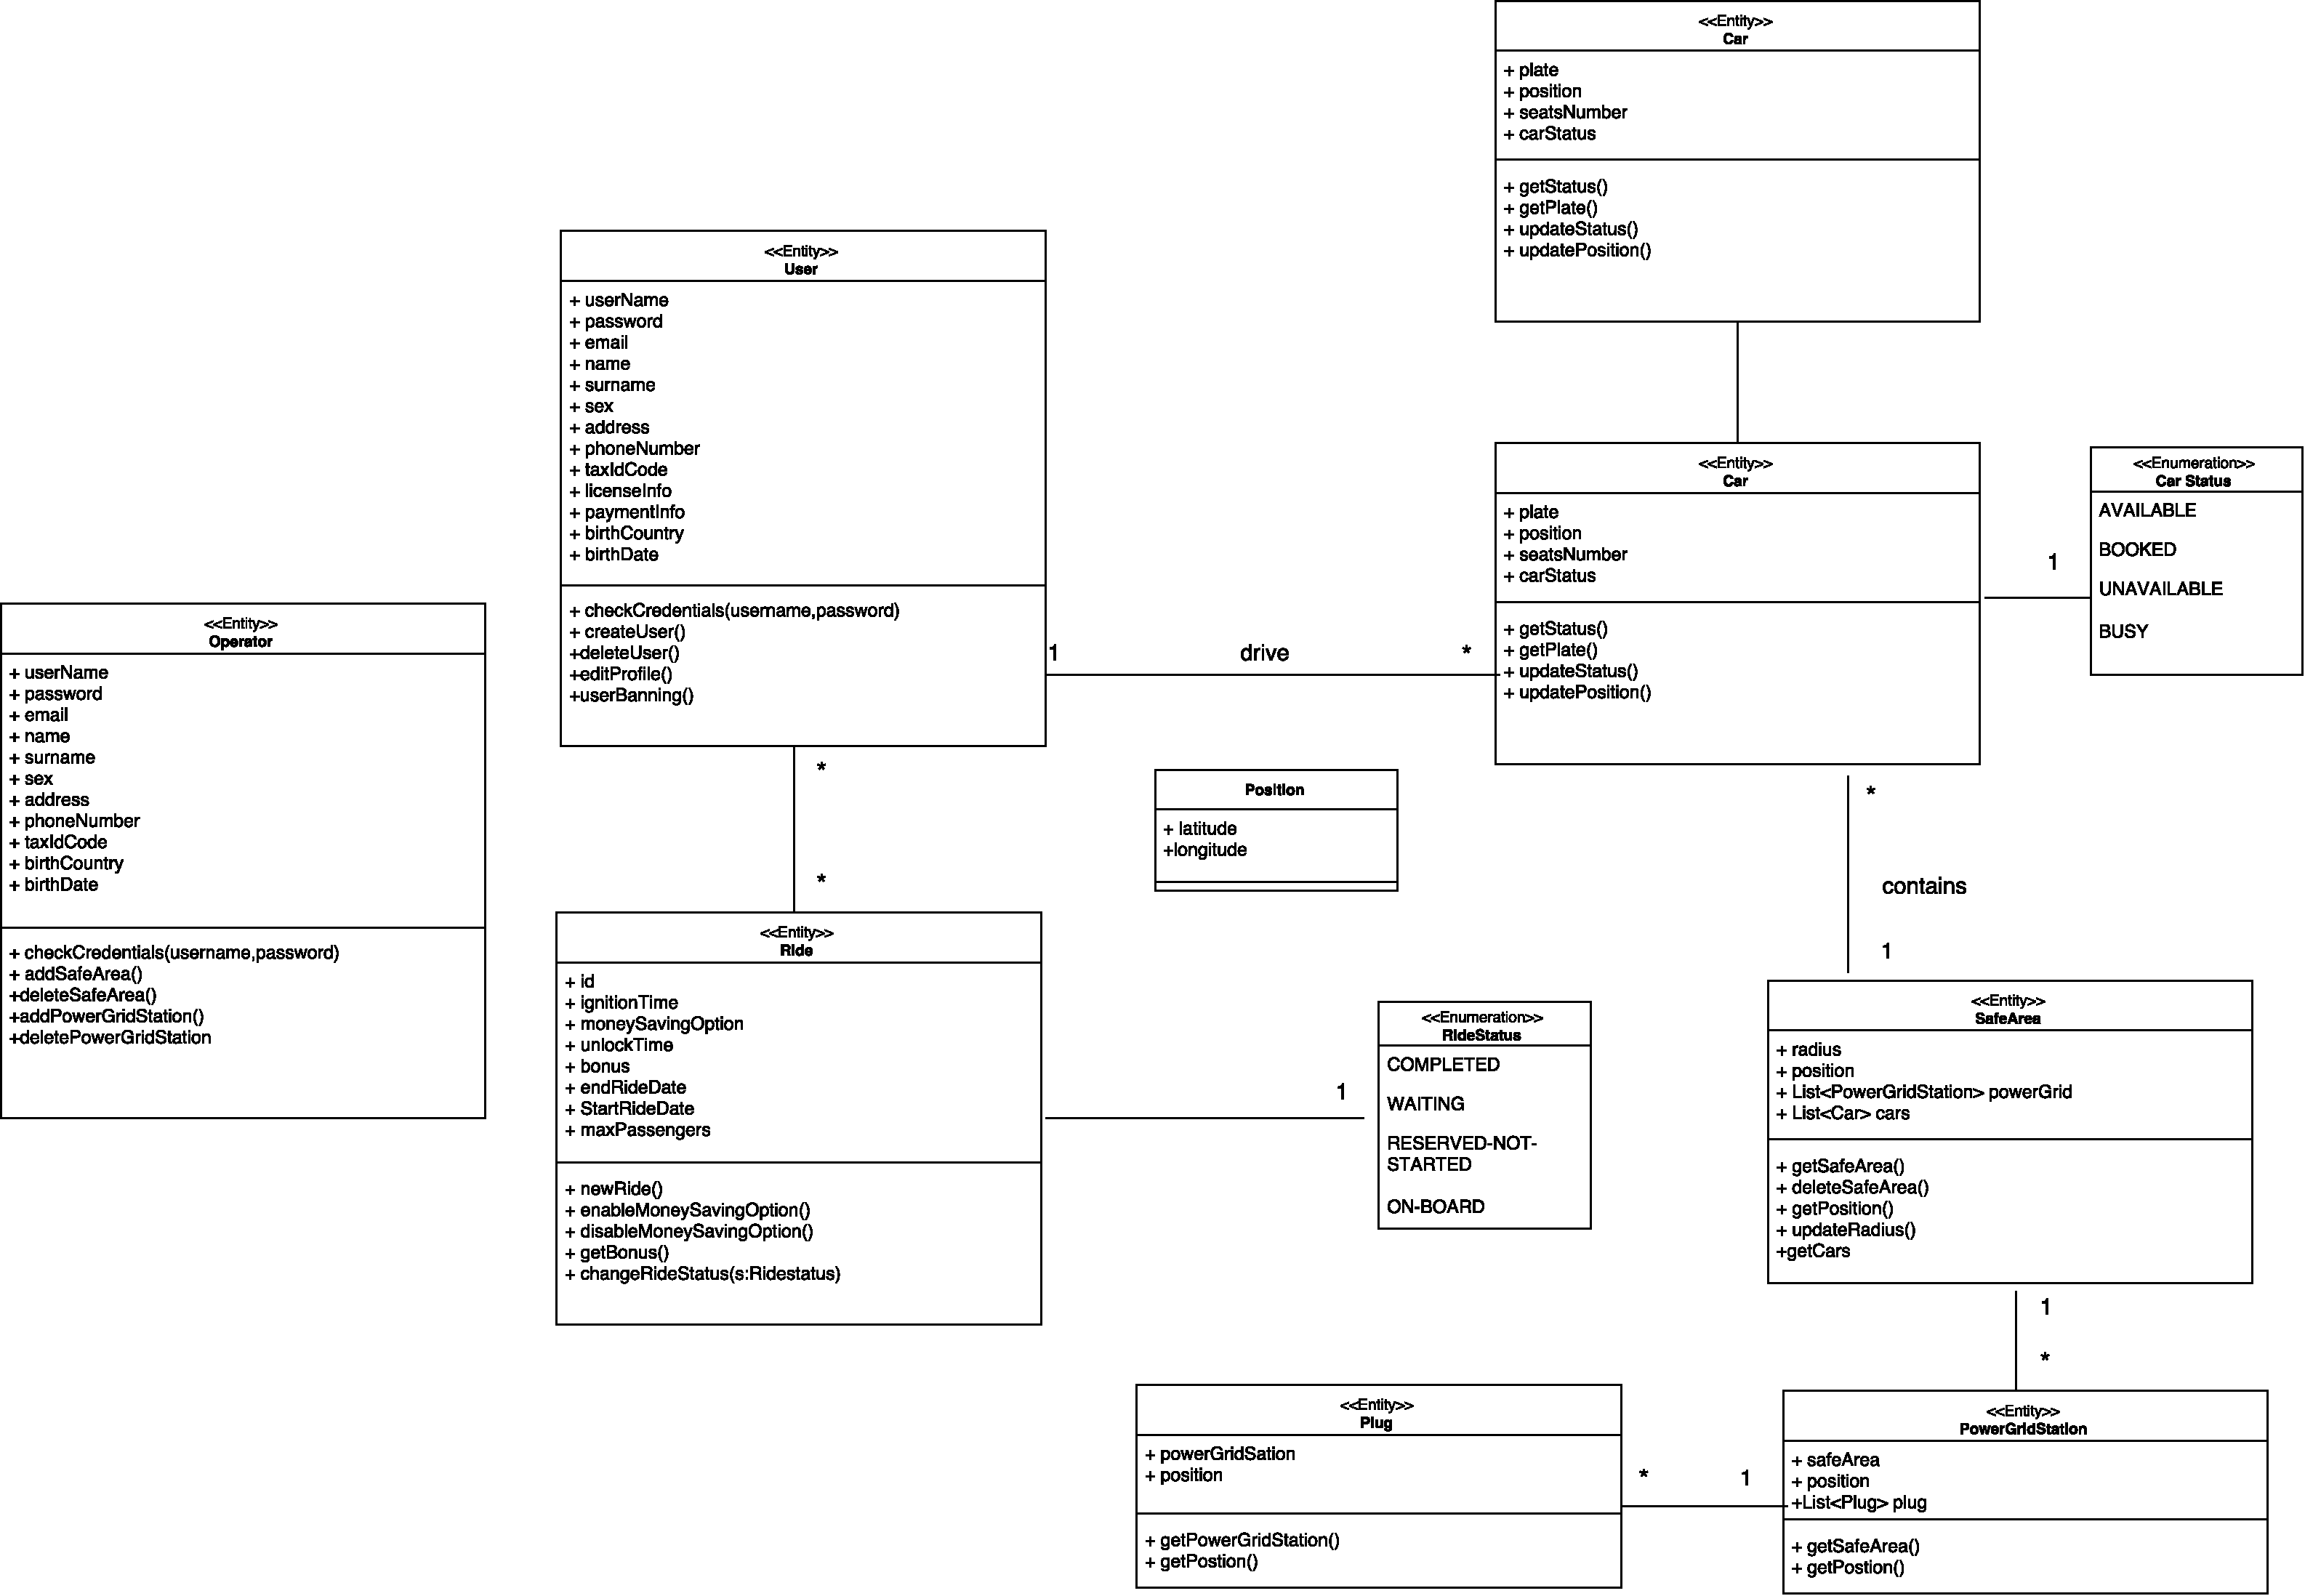
\includepdf{architectural_design/Architecture_Diagrams/EntityBeans.pdf}
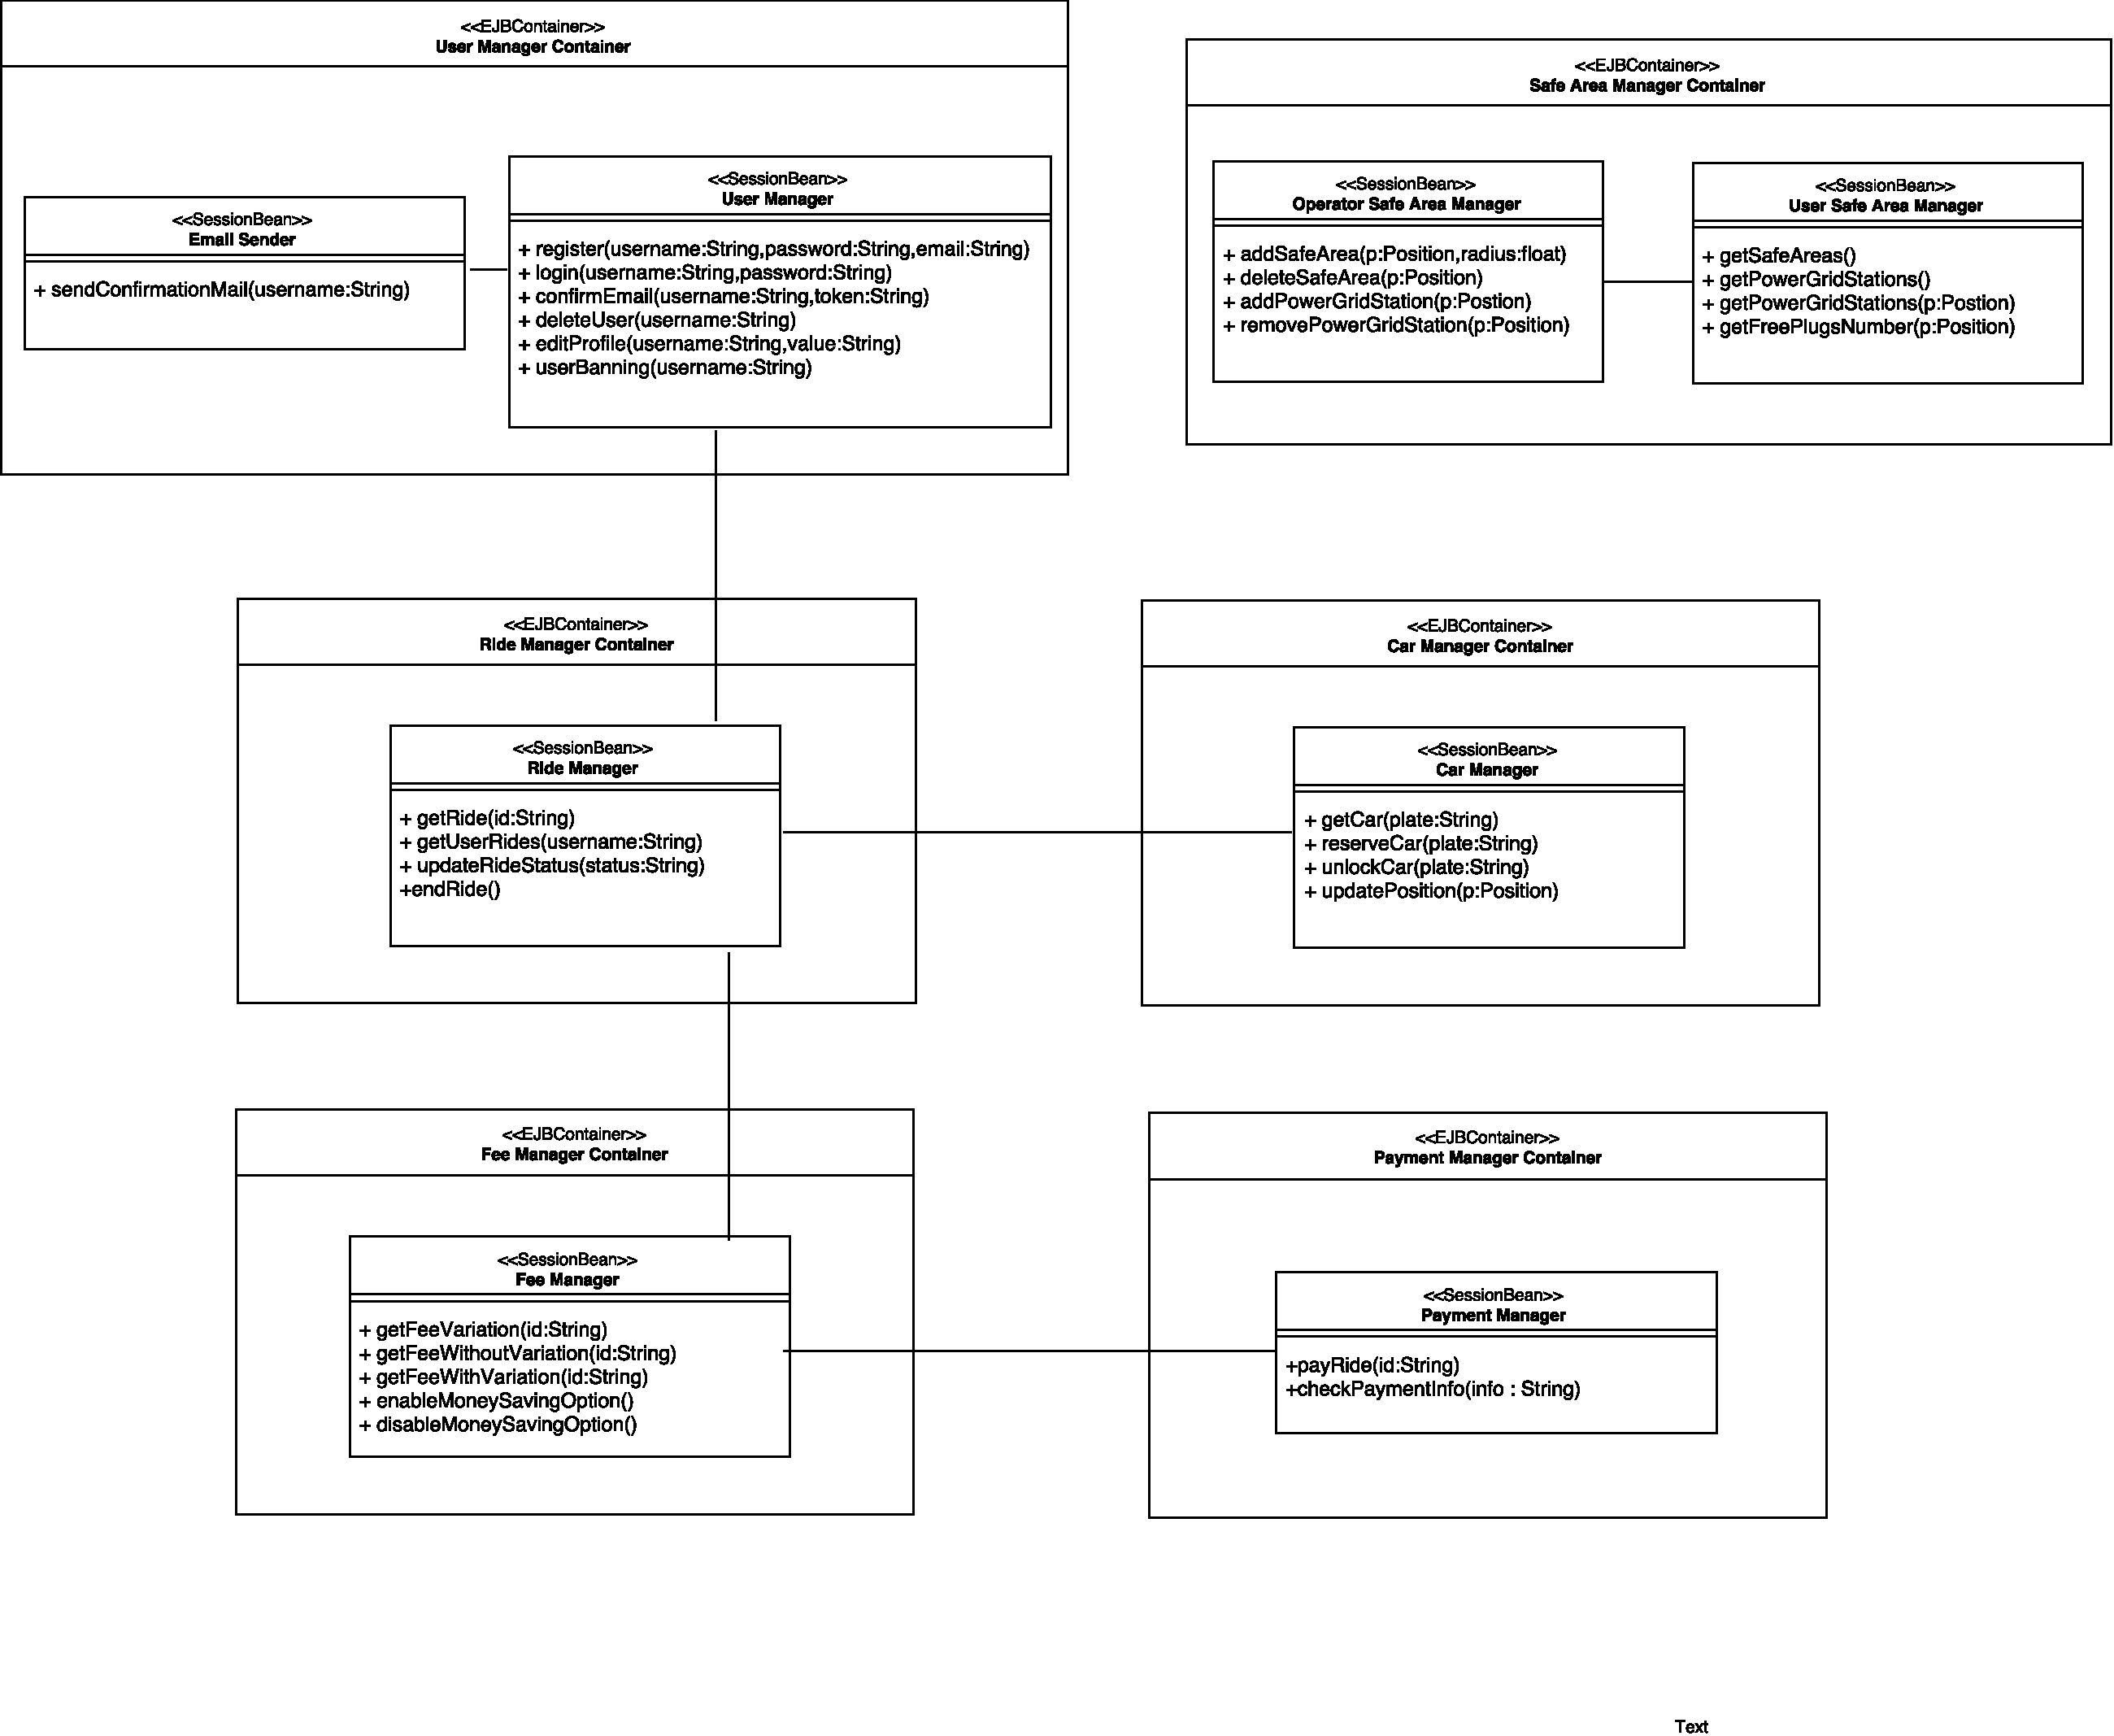
\includepdf{architectural_design/Architecture_Diagrams/SessionBeans.pdf}

\subsection{User Manager}
This bean manages all the user management features: user registration, user login user deletion, profile editing and user banning.
It also provides a function to confirm the email address provided by the user with the token sent by email.
This bean also communicate with two external systems:
\begin{itemize}
\item External Payment System that checks that the payment information provided by the user are correct and handle the payment process;
\item External System for Driving License Validation that check the driving license of the user during the registration process.
\end{itemize}

\subsection{Car Manager}
This bean manages manages all the car's features: get car, reserve car, unlock car and update position.
In this way it keeps references and update all the informations about the car, including the maximum number of passengers the battery level and the numbers of seats.
It also provides a function to handles the changes in the status of the car.

\subsection{Ride Manager}
This bean manages all the ride features:create new ride, get ride,get user's ride and end ride.
It provides functions that return all the rides informations like the number of passenger on the car,the unlock time and the user that has reserved the car.

\subsection{Fee Manager}
This bean manages all the functionalities about the fee of the ride: calculate fee variation, calculate fee with variation and calculate the fee without variation.
It handles all the information about the bill that the user has to pay and apply discounts when it is necessary.

\subsection{Safe Area Manager}
This bean allows the operator to manage the safe area and provides functions to add a new safe area and to delete it. It also provides function to add and delete a power grid station in a specific position.
Besides it offers also some function available also to the user that allows him/her to know the safe areas and power grid stations positions.

\subsection{Payment Manager}
This bean provide a function to pay the ride and another one to check the payment information provided by the user thanks to an external system of payment information validation.
\section{Deployment View}
The the business logic layer containing the application server is allocated on one physical machine (tier), while the data are on another dedicated machine. GlassFish Server is used as the Java EE application server for the business logic.
\section{Runtime View}

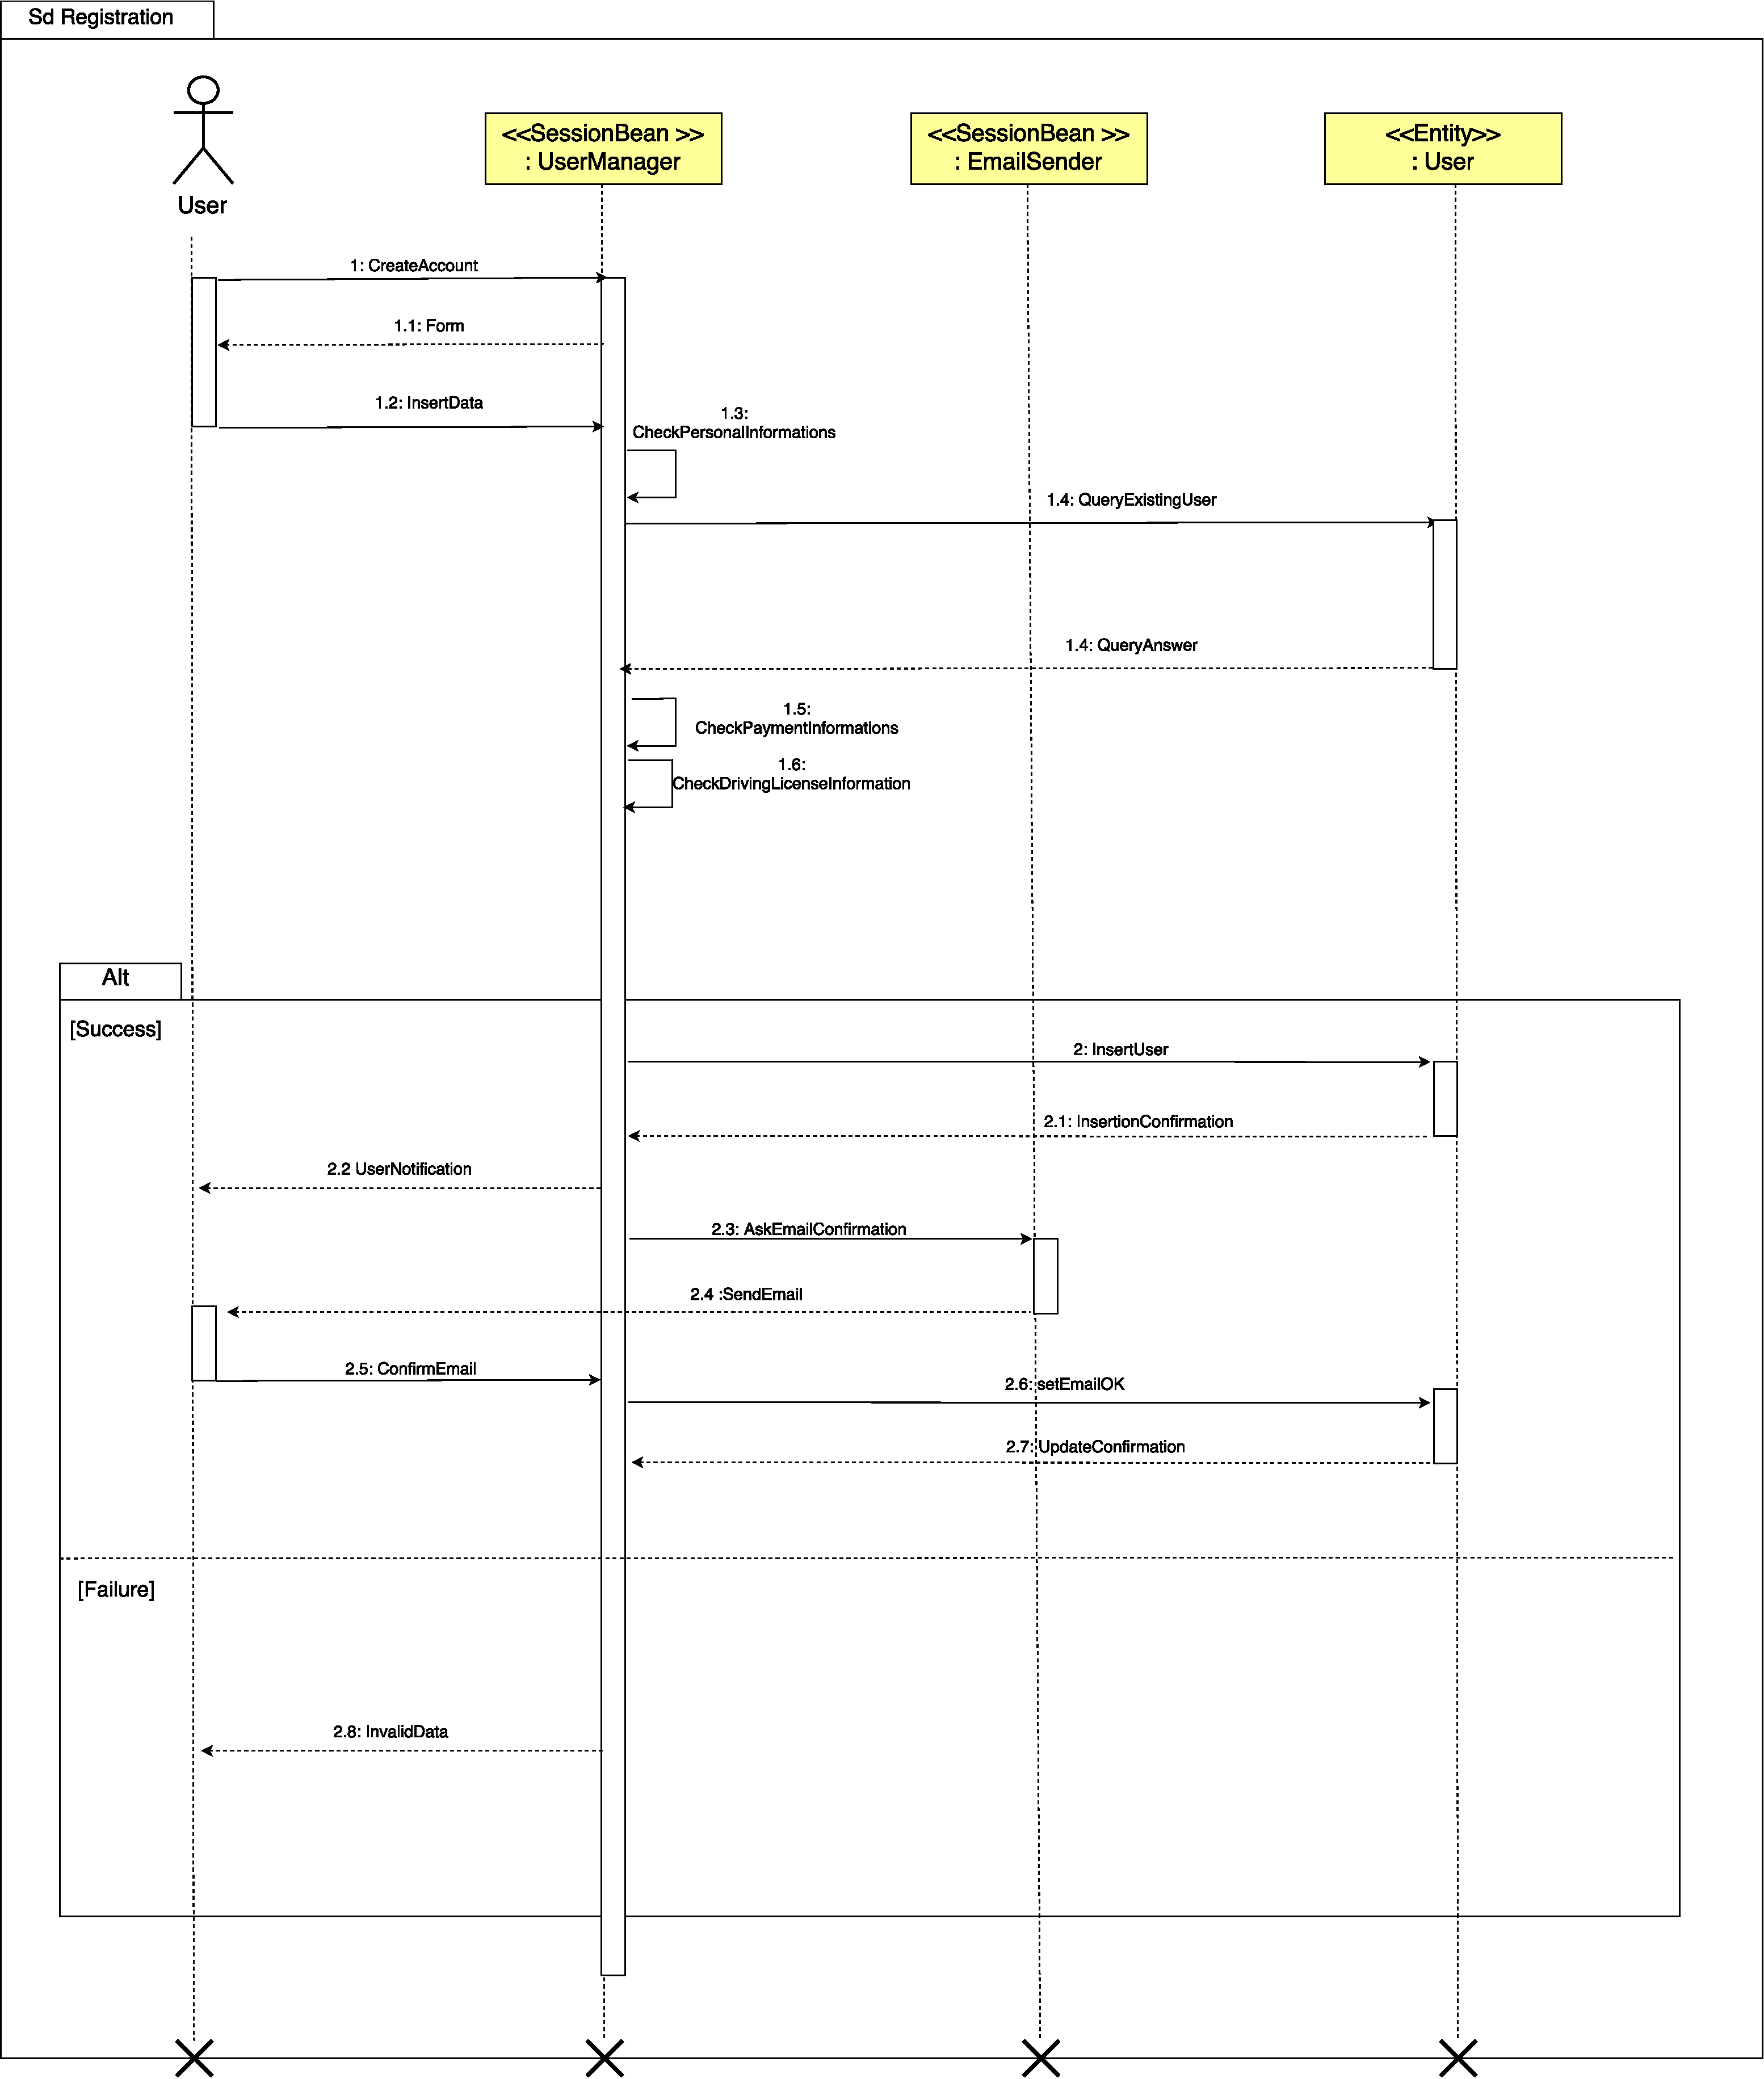
\includepdf{architectural_design/Architecture_Diagrams/RegSequence.pdf}
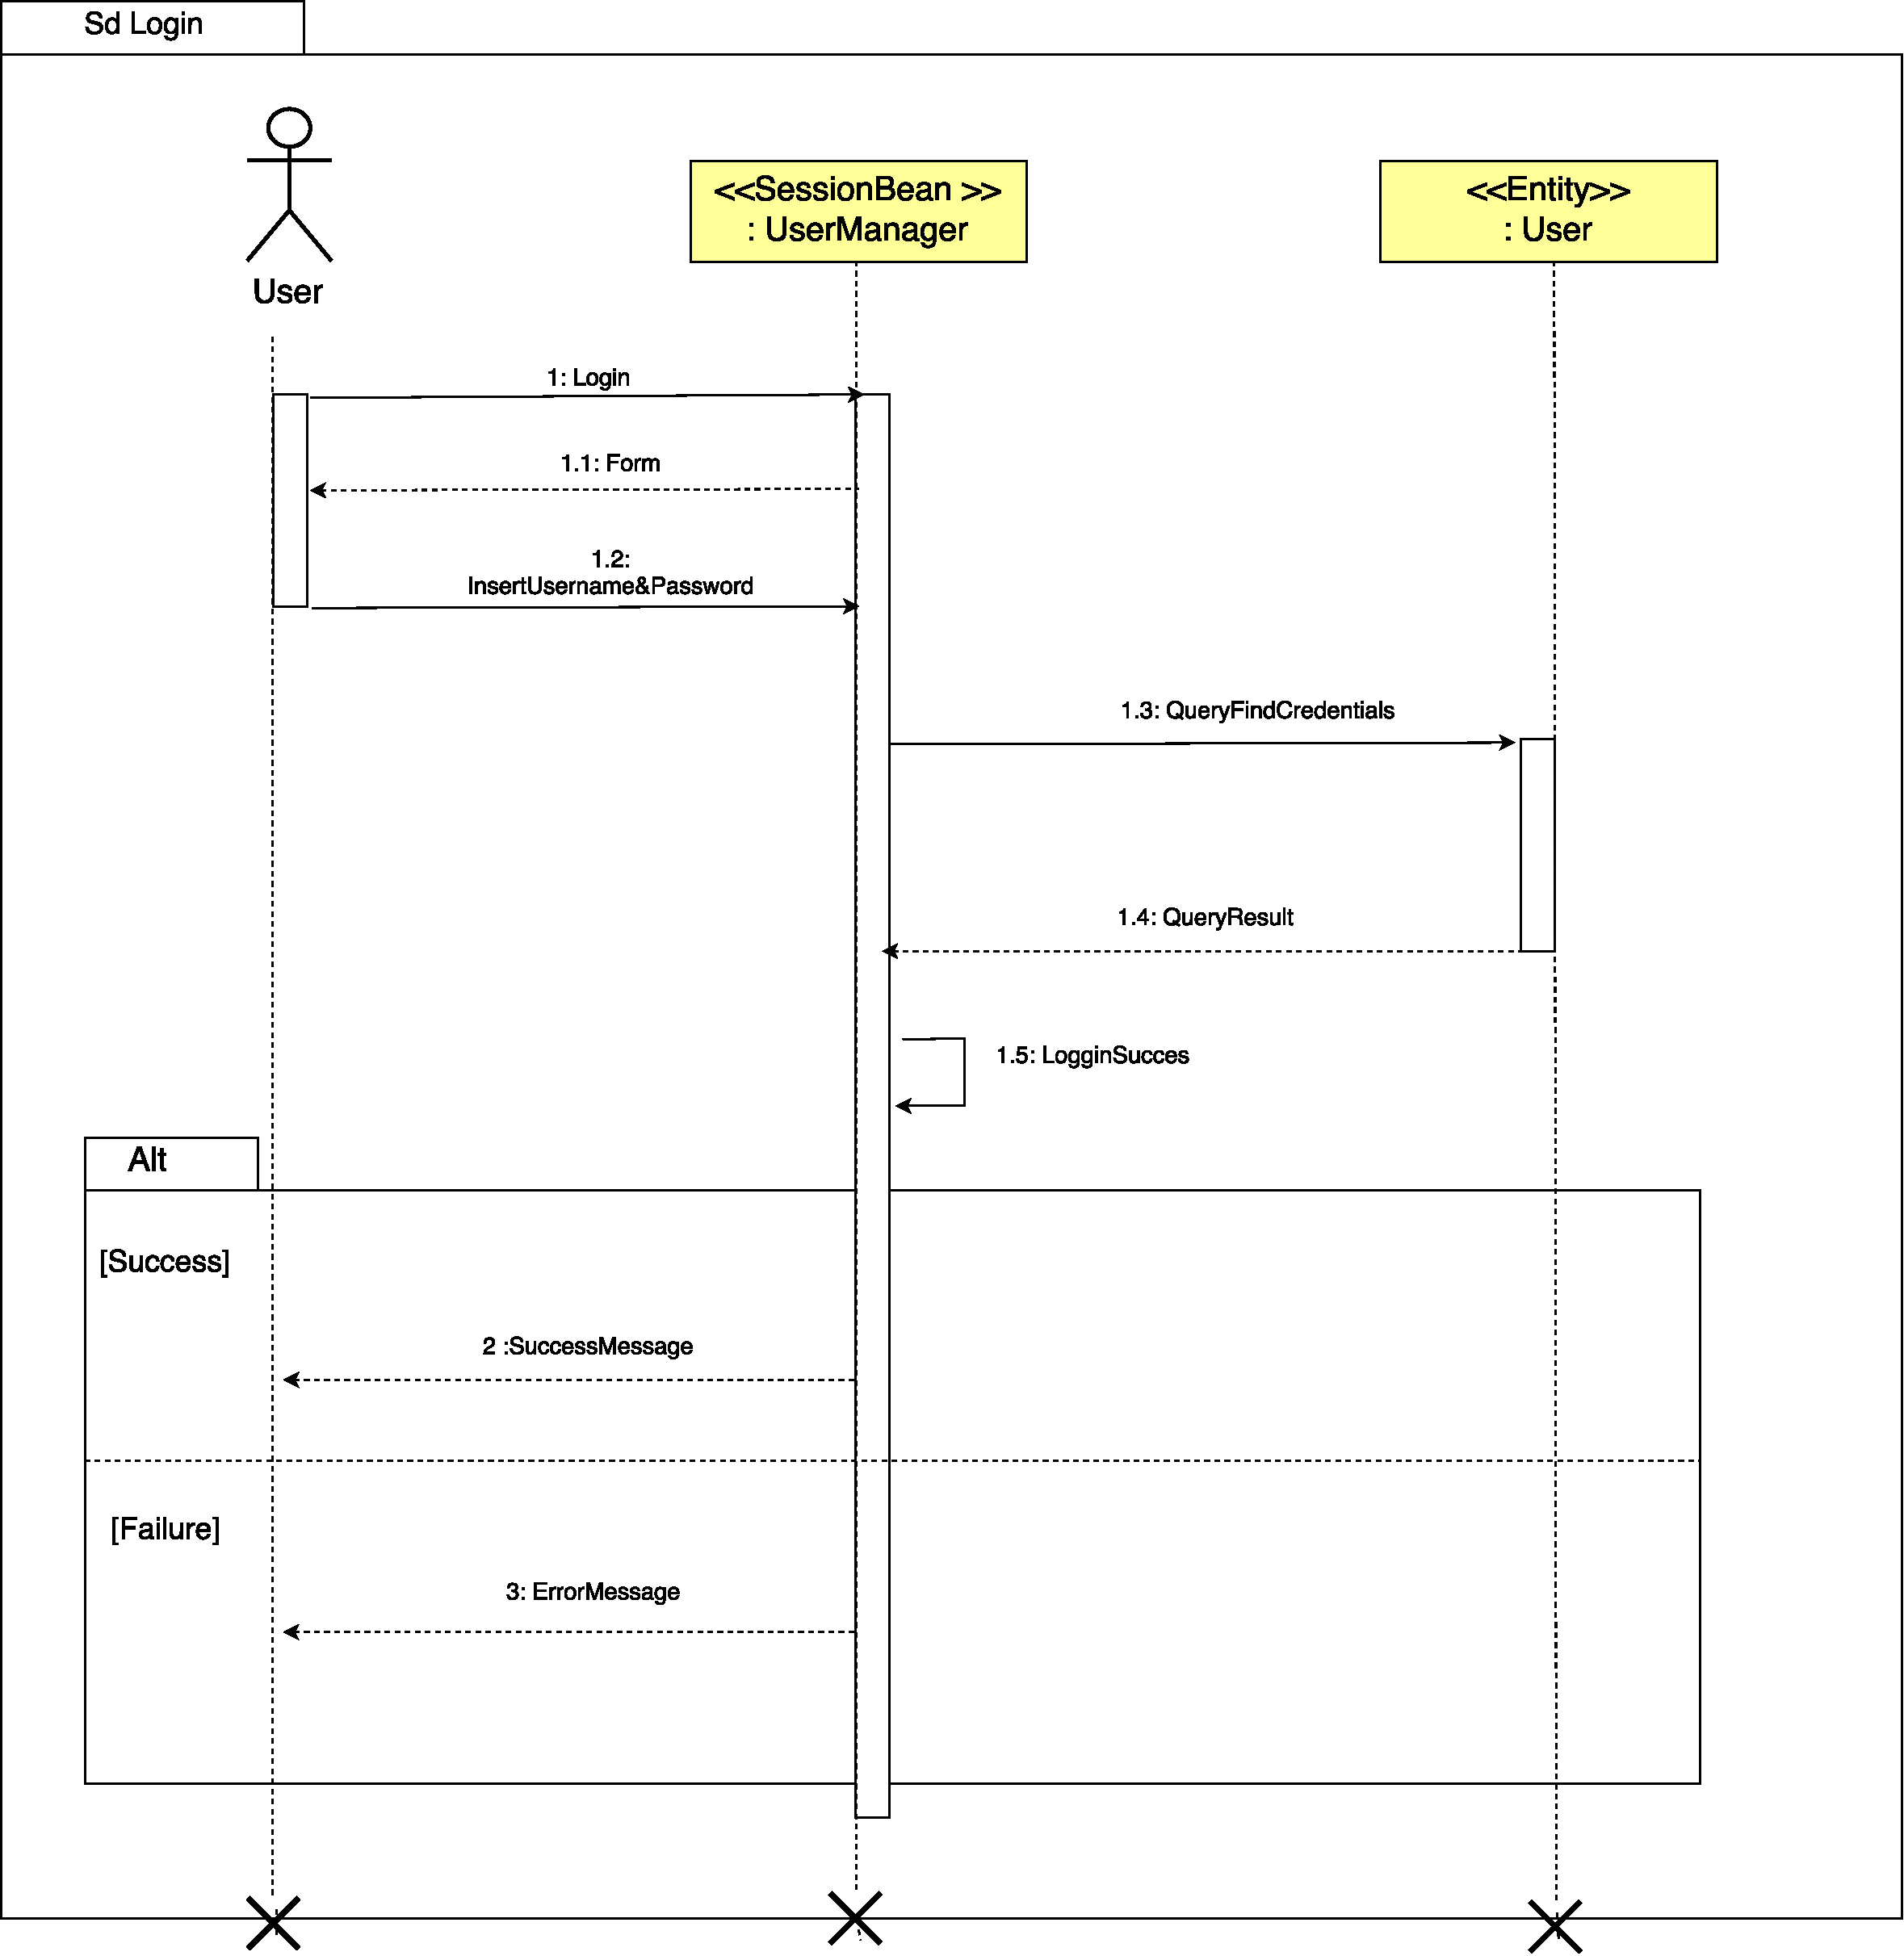
\includepdf{architectural_design/Architecture_Diagrams/LoginSeq.pdf}
\section{Component Interfaces}

\subsection{Logic layer to data storage layer}
The logic layer communicates with the data storage layer via the Java Persistence API (JPA) over standard network protocols.
In this way, the two layers can be deployed both in different tiers or in the same one.

The JPA specification uses an object/relational mapping approach to bridge the gap between an object-oriented model and a relational database in order to focus more on the object model rather than on the actual SQL queries used to access data stores.

\subsection{Logic layer to presentation layer}

The application server communicates with the other elements of the system through a RESTful interface over the HTTPS protocol.
The RESTful interface is implemented using JAX-RS and uses JSON as the language data format.

\subsubsection{User Manager}
All the following functions can be called by the mobile app of the user:
\begin{itemize}
	\item \textbf{void register(String username, String password, String email):} Add a new user in the system with the provided data if these are correct.
	After this, an email with a token is sent to the user email address in order to confirm the latter.
    \item \textbf{Token login(String username, String password):} Allows any registered user to log into the system using his own username and password.
    If these credentials are correct, the function returns a token to be used in the future requests to identify the user, otherwise it returns an error.
    \item \textbf{void confirmEmail(String username, Token emailToken):} Validates the email address that was inserted by a registered user using the token sent to that email address after the registration.
    \item \textbf{void deleteUser(String username, String password):} Allows users to delete the user account and information, except for his essential information and rides because they can be requested from authorities. As parameters it takes the username of the user and his password.
	\item \textbf{void editProfile(String fieldName, String newValue):} Allows users to edit their information. If they user wants to change its email, he/she has to confirm it as for the registration.
	\item \textbf{void userBanning(String username):} Blocks the user's account.% if he/she has some pending bills until it will be paid.
	This function is available only for PowerEnJoy operators.
	%\item \textbf{Driving license validation:} Check the validity of the driver license provided by the user through an external system.
	%\item \textbf{Payment information verification:} Check the correctness of the payment information provided by the user through an external system.

\end{itemize}

\subsubsection{Ride Manager}
\begin{itemize}
	\item \textbf{Ride getRide(String id):} Returns the ride info that corresponds to a given ID. The function will return an error if a user wants to retrieve the info about a ride that is not assigned to him/her.
	The PowerEnJoy operators can get all the rides, without restrictions.
	The info about a ride contain: the plate of the car, the username of the user that reserved the car, unlock time, ignition time, end time, the fee with variations and the fee variations and the maximum number of passengers.
%	\item \textbf{Add ride:} Registers a new ride with the start time, the unlock time, %TODO the ignition time, 
%the plate of the car and the username of the user.
	\item \textbf{List \textless Ride\textgreater{} getUserRides(String username):} Returns the rides info that corresponds to a given users. The function will return an error if a user wants to retrieve the info about another user.
	The PowerEnJoy operators can get all the rides, without restrictions.
\end{itemize}

\subsubsection{Car Manager}
\begin{itemize}
	\item \textbf{Car getCar(String plate):} Returns the car info that corresponds to a given plate.
	The info about a car contain: the battery level, the state, if the engine is on or off, the number of seats, the model and the manufacturer.
	\item \textbf{void reserveCar(String plate):} The mobile app calls this function to allow the user to request a car. This function returns an error if the request is not valid.
	\item \textbf{void unlockCar(String plate):} The mobile app calls this function to allow the user to unlock a car that he reserved. This function returns an error if the request is not valid.
%	\item \textbf{Update position:} Updates the position of the car. This function is called periodically to monitor the movements of the cars.
	\item \textbf{void endRide():} The HandyCar Board use this function to report to the system that the user ended a ride. At this point, the application server saves the end time, the fee variation that were applied and the maximum number of passengers. Every HandyCar Board has its own ID, so the system can recognize from which car the request is sent.
\end{itemize}

\subsubsection{Fee Manager}
All this functions can be called from the user of the ride or from PowerEnJoy operators.
\begin{itemize}
	\item \textbf{int getFeeVariation(String ID):} Calculates a fee variation for a given ride ID. 
	\item \textbf{int getFeeWithoutVariation(String ID):} Calculates a fee for a given ride, without including the variations of bonuses and penalty.
	\item \textbf{int getFeeWithVariation(String ID):} Calculates a fee for a given ride, including the variations of bonuses and penalty.
\end{itemize}

\section{Selected architectural styles and patterns}
%Please explain which styles/patterns you used, why, and how
We used the following architectural styles and patterns:

\begin{description}
\item[Client-Server:]
The client–server model is used between these communications:
	\begin{itemize}
    \item the application server (client) queries the DB (server);
    \item the presentation layer (client) communicates with the application server (server);
    \item the application server (client) and the on-board tablet (server);
    \item the HandyCar Board and the application server (both act like client and server);
    \item the application server (client) and the payment validation external system (server);
    \item the application server (client) and the driving license validation external system (server).
	\end{itemize}

We choose this type of architecture to have a centralized control and because it is simple and well known by our development team.

\item[Service-oriented architecture:]
The SOA is used by the system for the communication between the application server and the presentation layer.

We used SOA in order to have an high level interaction between these two layers, by looking only at the component interfaces, that represent a black box for its consumers.

In this way, a service logically represents a business activity with a specified outcome, so you want to use it, you do not have to look inside its specific implementation.

\item[Thin client:]
The thin client is implemented in the mobile app and in the on-board tablet.
We used this paradigm in order to have light-weight apps, that can run in a large number of devices with a smooth user interaction.

Instead, all the application logic is on the application server, on which the client depends heavily on.
This can help to reduce the number of updates, because if you want to change something in the application logic, it is not necessary to release a new application of the client.

\end{description}
% \subsection{Model-View-Controller}

\section{Other design decisions}
% not mandatory
other design decision


\chapter{Algorithm Design}
\label{ch:algorithm_design}
\section{Algorithms}
In this section we will describe some algorithms used by the system in different phases of car rent management. We cannot describe all the algorithms used by the system, due to its complexity. However we have chosen the most important ones, in order to show some development choices we made.
The chosen algorithms are these four:
\begin{enumerate}
\item Given a ride, calculate the final fee
\item Given a circle with center c and radius r, find all the Safe Areas that intersect the given circle
\item Given a position, find all the car far at most 2km
\item Given a destination, find the Safe Area where to park
\end{enumerate}
In the algorithm description there is not the final code. Instead we will use a mix of common speech and pseudo-code (easy to translate into the desired programming language). This pseudo-code is referred to an object-oriented programming language.

\subsection{Algorithm 1: How to calculate the final fee}
When a ride ends it is important to calculate the final fee to charge to the user. This may differ to the amount shown on the car screen due to some bonus or malus (called fee variator) unlocked by the user.
This function will be called by the server once a ride ends. It will have a ride in input and a float as output, that represents the final fee to charge.
Just to remember, a ride has the following fields:
\begin{itemize}
\item Reservation Time
\item Unlock Time
\item Ignition Time
\item End Time
\item User
\item Car
\item max Passengers Number
\item a set in which are stored the fee variator already unlocked
\end{itemize}

We also remember that each fee variator has a float field that represents the percentage variation made by that fee variator. These float is positive for the malus (because it has to increase the fee) and is negative for the bonus (because it has to reduce the fee).

In order to describe the algorithm in the easiest way we assume:
\begin{itemize}
\item the function can accede to the cost per minute of the rent (CPM) and a set of all the fee variator that can be unlocked (called feeVariatorSet)
\item the difference between two dates is the number of minutes between them
\item each fee variator has a function check(Ride ride). Given a ride this function returns true if the relative fee variator can be unlocked, false otherwise.
\end{itemize}

\begin{algorithm}[H]
	\SetKwInOut{Input}{Input}
    \SetKwInOut{Output}{Output}
   % \SetKwData{ADD}{add}\SetKwData{ALL}{all}\SetKwData{IN}{in}
\SetKwData{Var}{var}\SetKwData{FVS}{feeVariatorSet}\SetKwData{Ride}{ride}\SetKwData{Res}{result}\SetKwData{cpm}{CPM}
\SetKwFunction{check}{check}\SetKwFunction{RL}{rideLenght}

	\Input{A ride}
	\Output{The final fee to charge}
	\BlankLine
\ForEach{\Var in \FVS}{
\lIf{\Var .\check{\Ride}}{
add \Var in \Ride .feeVariator 
}}
	\BlankLine
\Res = \RL{\Ride} * \cpm \;
	\BlankLine
\ForEach{\Var in \Ride .feeVariator}{
\Res = \Res + \Res * \Var .variator \;
}
\Return \Res \;
\caption{How to calculate the final fee of a ride}
\end{algorithm}


 

\chapter{User Interface Design}
\label{ch:ui_design}
\section{User Experience}
We have already dealt with user interface designs in the RASD, where we have shown some mock-ups of the screens of our application.

In this section we will model the user experience, showing how the interface changes with the input of the user and external factors, so we will map the sequence of actions and events with the screens flow.

We will use the class diagram for the user experience modelling. This approach needs some clarification about the used notation, so below we are going to explain the meaning of the symbols used:

\begin{description}
\item[Directed arrow:] It defines a transition from a particular user interface element to another. It may be due to two possible cause:
	\begin{description}
	\item[User input:] This type of transition is triggered by the invoking of a particular method \textit{function()} in the source interface element.
	The name of the user input transaction is the same of the function that was invoked by the user. Sometimes the method can rise an error, so in these cases the name of the transaction is followed by "ok" if the outcome of the function is positive or by "error" if it is negative. 
	\item[Event:] This type of transition is triggered by an event that can be generated by the client itself or by a message sent  by the server to the client. This transaction is identified by the "event" at the end of the name.
	\end{description} 
\item[Class symbol:] It determines a specific user interface element among \textit{Screen}, \textit{Input form}, \textit{Element}, \textit{Pop-up}\ and \textit{Frame}
or a specific event (stereotype \textit{event}). In both cases the type of element is specified in the stereotype of the class symbol. 
\item[Composition symbol:] Means that a specific user interface element is contained in another. Typically is used when a form or a list of elements is contained in a particular screen. It can be also used to say that a generical user interface element displays some info.
\end{description}

It is important to underline that, in order to maintain readability, only the main elements are shown in the following diagram.

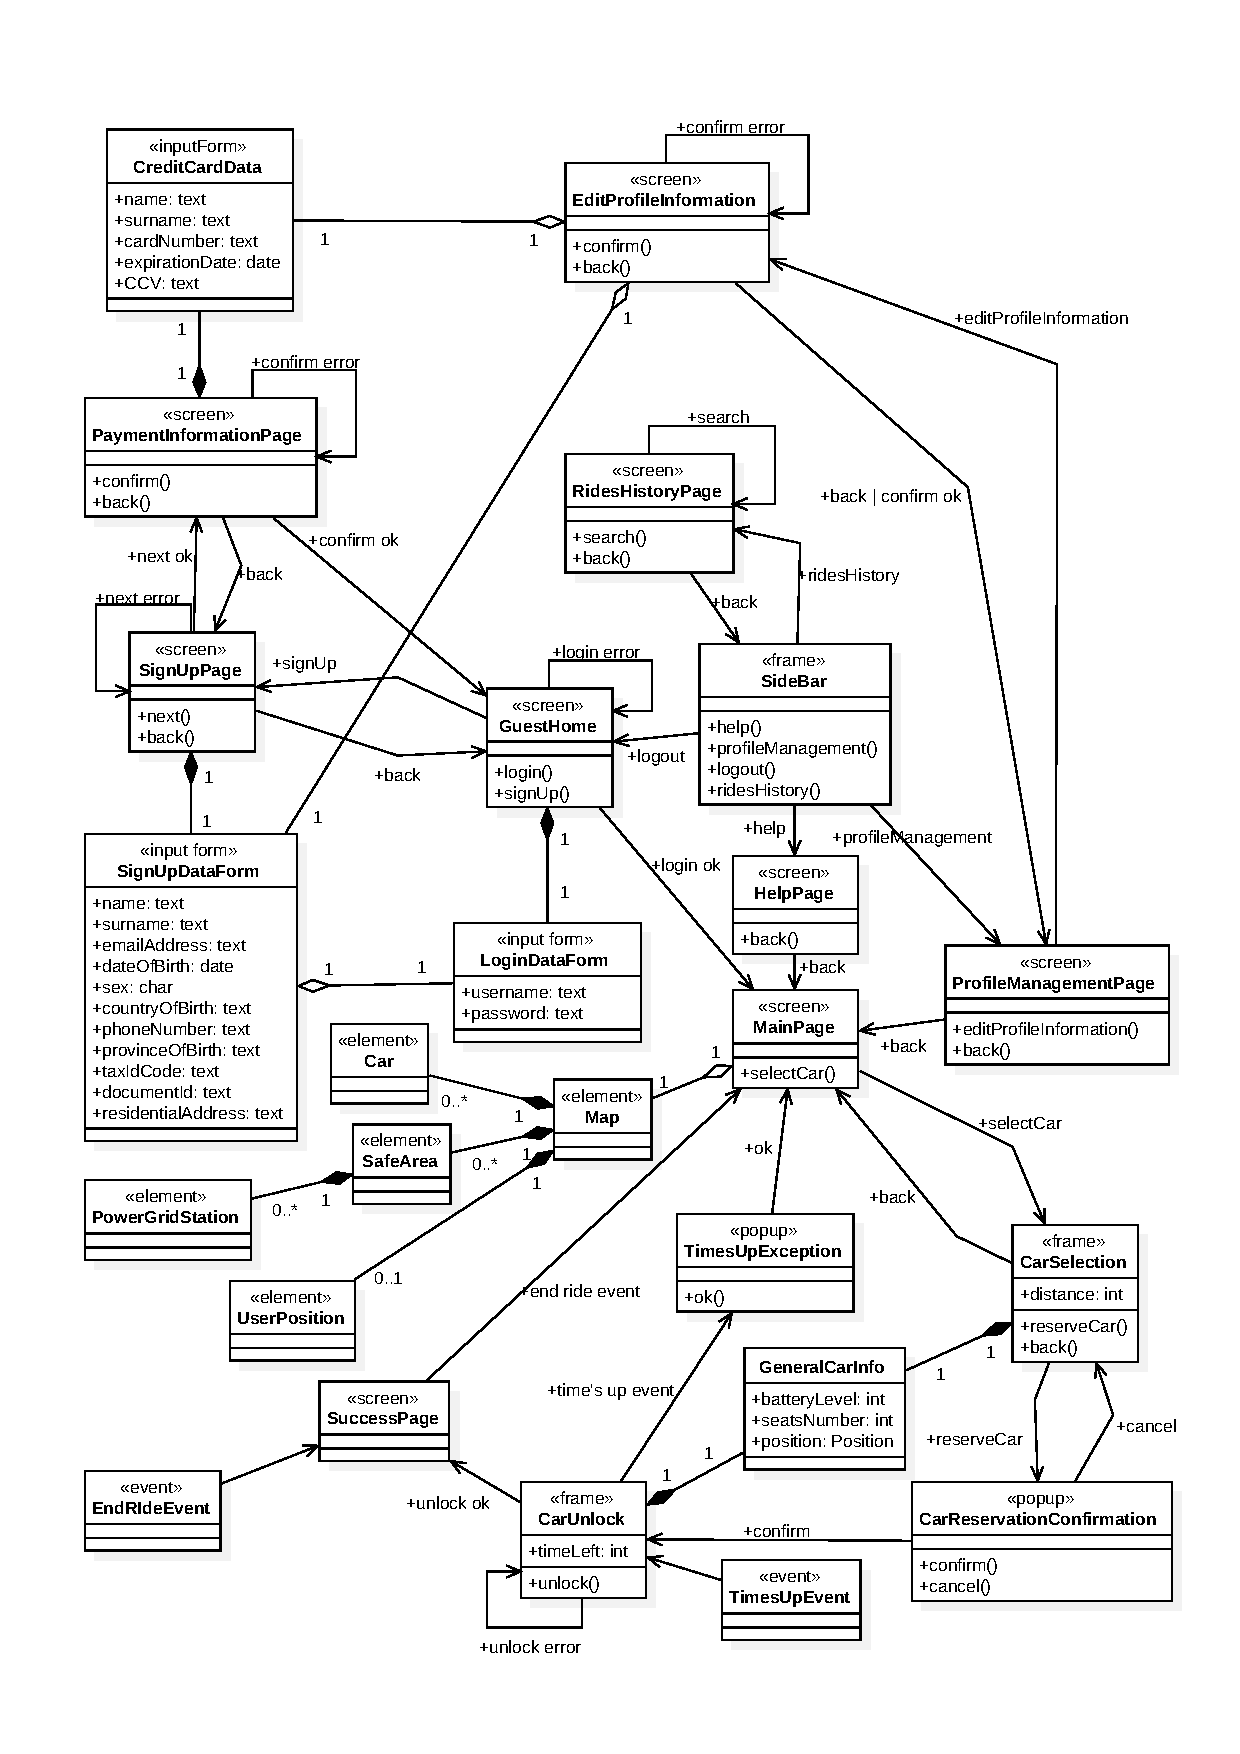
\includepdf{ui_design/user_experience.pdf}

\section{Car Tablet}
We have already shown the mobile app user interface in the RASD, so in this section we will show some mock-ups of the tablet that is present in every car.

\begin{figure}
    \vspace*{-2cm}
    \makebox[\linewidth]{
        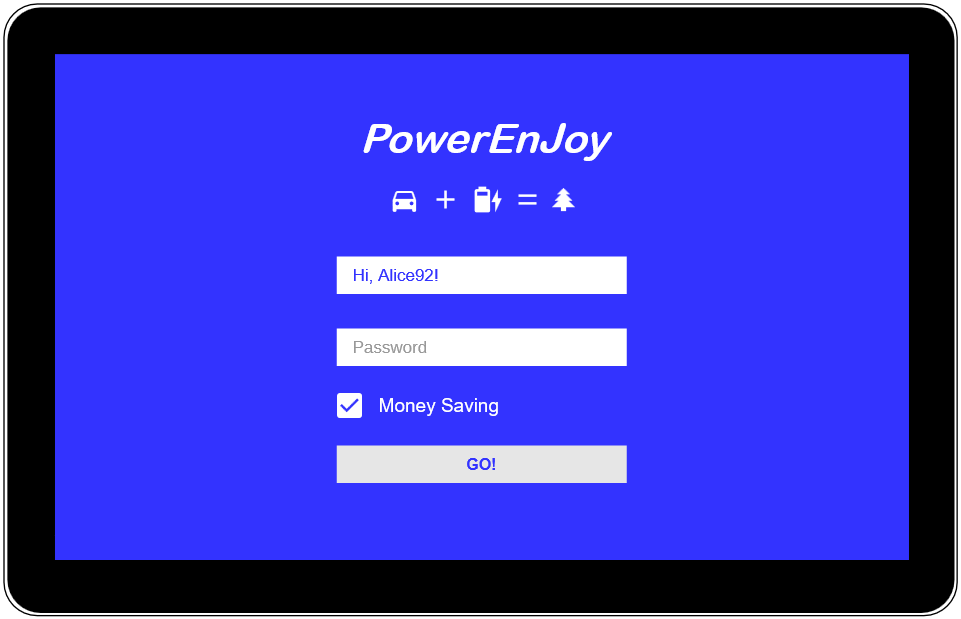
\includegraphics[width=1.3\linewidth]{ui_design/car_login.png}
    }
    \caption{Car login page.}
	\label{fig:car_login}
\end{figure}

When the user enters the car, the screen in figure \ref{fig:car_login} is what he/she will see in the tablet. The tablet receives the nickname of the user that unlocked the car, so it is able to display it. If the password is correct than the user can turn on the car.

\begin{figure}
    \vspace*{-2cm}
    \makebox[\linewidth]{
        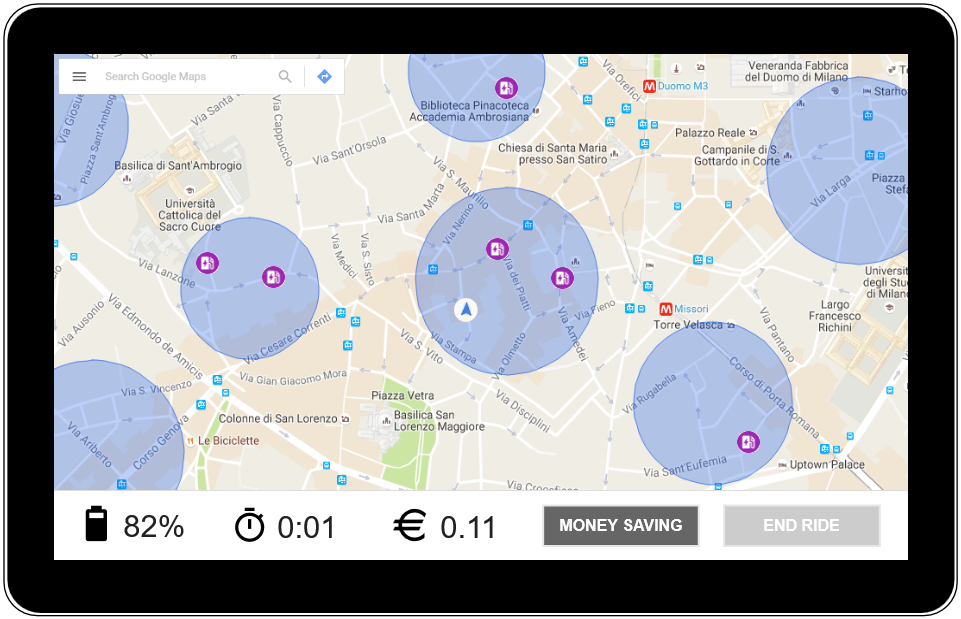
\includegraphics[width=1.3\linewidth]{ui_design/car_main.png}
    }
    \caption{Car main page.}
	\label{fig:car_main}
\end{figure}

If the authentication phase is successful, then on the tablet appears the Main Page. The mock-up of this screen is presented in figure \ref{fig:car_main}. Here you can navigate through the map, where you can find also the safe areas and the power grid stations. In the bar at the bottom, you can find the current percentage of the battery level of the car, the time since the reservation started, the current fee and the buttons to activate the money saving option and to end the ride.

In this picture the money saving option is off and the end ride is disabled because the user is not in a safe area. When the user is in a safe area the button becomes red. Using the search bar, the user can select a destination and set the navigation.

If he/she do so, the screen of the tablet will be something similar to figure \ref{fig:car_ride}. In this example the money saving button is blue, so it means that this option is activated.

\begin{figure}
    \vspace*{-2cm}
    \makebox[\linewidth]{
        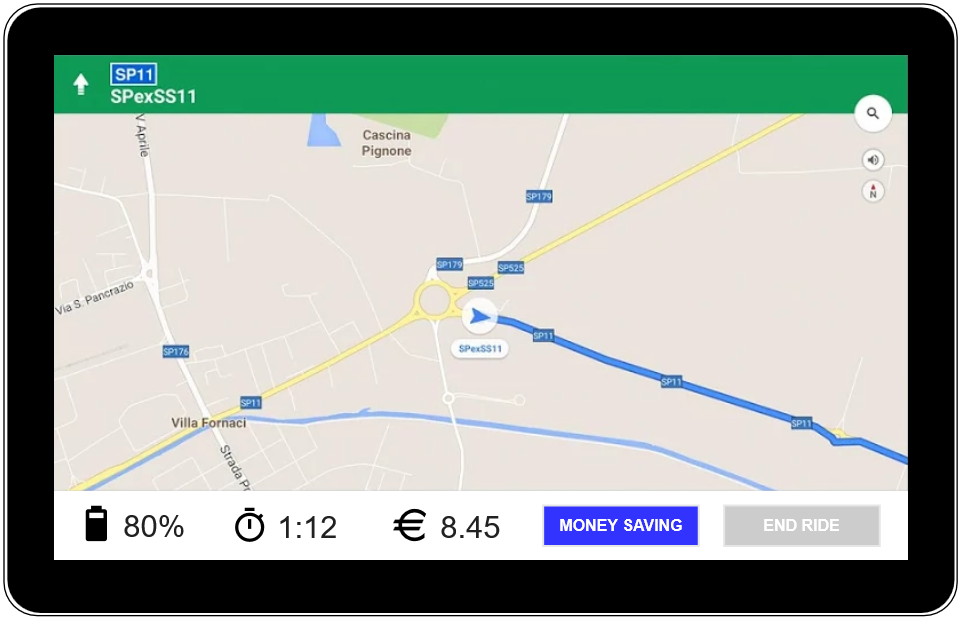
\includegraphics[width=1.3\linewidth]{ui_design/car_ride.png}
    }
    \caption{Car main page.}
	\label{fig:car_ride}
\end{figure}


\chapter{Requirements Traceability}
\label{ch:requirements_traceability}


\end{document}
